\section{Practical}
	\subsection{Creating the The App}
		CI/CD was demonstrated using a simple web app. The objective was to create a web app which can be continuously deployed to AWS. For demonstration purposes a very basic app was created using NodeJS library ReactJS. It is simply a frontend web app that displays a basic ReactJS homepage as a visual indication of a successful deploy. The app running locally can be seen in \autoref{fig:app-local}.
		\begin{figure}[H]
			\caption{React App}
			\centering
			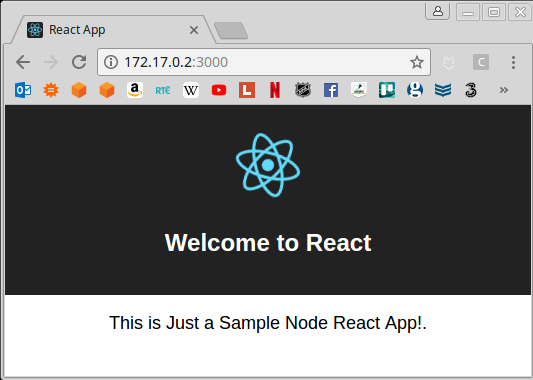
\includegraphics[width=\textwidth,keepaspectratio]{app-local}
			\label{fig:app-local}
		\end{figure}
		In order to implement continuous integration, the app will be built by means of a Docker image which can be pushed to a Docker Hub registry. True continuous integration would often also implement testing before building the image\citep{docker}. However, as this is just a basic sample app no tests are included.
		
		To \textit{dockerise} the image a \textit{Dockerfile} was added to the source code. This \textit{Dockerfile} specifies a base image for the file (a standard node image for Docker Hub) and copies the source code into the image. It installs the necessary software (npm) and starts the app. It is worth noting that this is starting the app in development mode as opposed to building the app with \textit{npm build} as this is just for demonstration purposes. The \textit{Dockerfile} also exposes port 3000 of the container. This is the port on which the app run in development mode and can be observed in \autoref{fig:app-local}. Later, when the image is run on an ECS instance, this container port will need to be mapped to a host port on the instance.
		
		\begin{minipage}{\textwidth}
		\begin{lstlisting}[caption={Dockerfile}]
		FROM node:carbon
		WORKDIR /usr/src/app
		COPY package*.json ./
		RUN npm install
		COPY . .
		EXPOSE 3000
		CMD ["npm", "start"]
		\end{lstlisting}
		\end{minipage}
	
	\subsection{Initial AWS setup}
		Some initial setup of AWS infrastructure was needed before the Jenkins job could run.
	
		\subsubsection{IAM Resources}
		The following IAM resources were needed for the project:
		\medbreak
		\noindent \textbf{Jenkins User:} As part of the build process the Jenkins job will execute a number of AWS CLI commands:
			\begin{itemize}
				\item Create an ECS Task Definition;
				\item Describe an ECS Task Definition;
				\item Update and ECS Service;
				\item Describe an ECS Service.
			\end{itemize}
		The most secure method of allowing this was to create an IAM user for Jenkins. Also created were two policies which together allow only the above actions. he policies were attached to the Jenkins user. An Access Key was generated for the Jenkins user to perform AWS CLI commands.
			
		\begin{minipage}{\textwidth}
		\begin{lstlisting}[caption={Task Definition Policy}]
		{
			"Version": "2012-10-17",
			"Statement": [
				{
					"Sid": "VisualEditor0",
					"Effect": "Allow",
					"Action": [
						"ecs:UpdateService",
						"ecs:DescribeServices"
					],
					"Resource": "*"
				}
			]
		}
		\end{lstlisting}
		\end{minipage}
					
		\begin{minipage}{\textwidth}
		\begin{lstlisting}[caption={Service Policy}]
		{
			"Version": "2012-10-17",
			"Statement": [
				{
					"Sid": "VisualEditor0",
					"Effect": "Allow",
					"Action": [
						"ecs:RegisterTaskDefinition",
						"ecs:DescribeTaskDefinition"
					],
					"Resource": "*"
				}
			]
		}
		\end{lstlisting}
		\end{minipage}
		
		\noindent \textbf{ECS Instance Role:} This role was created and the predefined policy \textit{AmazonEC2ContainerServiceforEC2Role} attached to it. The EC2 instance on which the app runs is registered to an ECS cluster. It uses an ECS agent to register to the cluster upon creation. In order for the agent to do so, it must communicate with ECS via an API call \citep{aws-agent}. This policy is used to grant and instance permission to communicate and interact with resources within ECS.
					
		\subsubsection{ECS Cluster}
		 An ECS cluster is a grouping of ECS instances. It allows scaling and load balancing of service such as a web app running in containers on multiple instances. As part this paper, autoscaling and load balancing are not implemented, however, they could be easily added by configuring an Application Load Balancer and configuring the ECS Service to autoscale on some configured Cloudwatch alarms. This is not necessary however for the demonstration purpose of this paper. However, an ECS cluster must still be created, with the instance running the app registered to it.
			
		\begin{minipage}{\textwidth}
		\begin{lstlisting}[caption={Create ECS Cluster},language=bash]
		aws ecs create-cluster --cluster-name $CLUSTER_NAME
		\end{lstlisting}
		\end{minipage}
		
		\subsubsection{EC2 Instance}
		This is where the app runs, albeit within a container. The instance must be an ECS optimised instance. This means it includes the ECS agent, a tool which runs on the instance allowing it to register with the cluster \citep{aws-instance}. It registers with the cluster by way of user data.
		
		\begin{minipage}{\textwidth}
		\begin{lstlisting}[caption={Create EC2 Instance},label={create-instance},language=bash]
		aws ec2 run-instances --image-id $AMI_ID --count 1 --instance-type t2.micro --key-name $KEY_NAME --security-groups $HTTPSSH_SEC_GROUP $HTTP_GITHUB --iam-instance-profile Name=$ECS_INSTANCE_ROLE --user-data file://user-data --tag-specifications 'ResourceType=instance,Tags=[{Key=Name,Value='$INSTANCE_NAME'}]'
		\end{lstlisting}
		\end{minipage}
		
		\begin{minipage}{\textwidth}
		\begin{lstlisting}[caption={User Data},language=bash]
		#!/bin/bash	
		echo ECS_CLUSTER=node-app-cluster >> /etc/ecs/ecs.config	
		\end{lstlisting}
		\end{minipage}
		
		Notice in \autoref{create-instance} that the instance is configured with the ECS Instance Role. By assigning this IAM role to the instance, it is able to assume the role, thus granting it permission to issue commands to ECS such as the necessary \textit{Register Container Instance}.
			
		\subsubsection{Task Definition}
		The task definition contains instructions on running the app. For example, the image to use and from where to pull it. In this case, the image is pulled from a registry on Docker Hub.
		
		\begin{minipage}{\textwidth}
		\begin{lstlisting}[caption={Task Definition Template},label=task-def]
		{
			"family": "node-app",
			"volumes": [
				{
				"name": "my-vol",
				"host": {}
				}],
			"containerDefinitions": [
				{
					"environment": [],
					"name": "node-app",
					"image": "rshelly/sample-node-app:v_%BUILD_NUMBER%",
					"cpu": 10,
					"memory": 500,
					"portMappings": [
						{
							"containerPort": 3000,
							"hostPort": 80
						}],
					"mountPoints": [
						{
							"sourceVolume": "my-vol",
							"containerPath": "/var/www/my-vol"
						}],
					"essential": true
				}]
		}	
		\end{lstlisting}
		\end{minipage}
		
		Notice in \autoref{task-def} the build number parameter is specified as the tag for the image. This is used because every time the Jenkins job runs, building the latest image, it will tag it with a version number (i.e. the build number). The task definition must specify that this latest image is to be used. Therefore, this task definition serves as a template for the Jenkins job to create up-to-date definitions every time a new image it built. For this reason, this task definition template was also placed on the Jenkins server where the job will have access to it.
		
		Also specified in the task definition is the port mapping. The container port is configured as port 3000 as this is the port on which the \textit{Dockerfile}, created above, exposes the app. This is mapped directly to host port 80, as not scaling is being implemented.
		
		As the Jenkins job has not run yet, there is no image in the registry yet. A dummy task definition with a build number of zero was registered with the cluster during the initial build.
		
		\begin{minipage}{\textwidth}
		\begin{lstlisting}[caption={Register Task Definition},language=bash]
		sed -e "s;%BUILD_NUMBER%;0;g" ./node-app.json > ./node-app-v_0.json
		aws ecs register-task-definition --cli-input-json file://node-app-v_0.json	
		\end{lstlisting}
		\end{minipage}
		
		\subsubsection{Service}
		An ECS service runs the task definitions. It also takes care of scaling and load balancing. If these were implemented it would have been a simple addition to the service of adding the Application Autoscaling Policy and registering a Target Group for the instance(s).
		
		Every time a new image is built, Jenkins creates a new task definition to run the newly built image from the Docker Hub registry. It then updates the service to run the new task definition in place of the old one. Therefore, the service must be created on ECS before the first run of the job. However, because no images have been built yet, it is configured with a desired count of zero. I.e. it will not run any task definitions.
		
		\begin{minipage}{\textwidth}
		\begin{lstlisting}[caption={Create Service},language=bash]
		aws ecs create-service --cluster $CLUSTER_NAME --service-name node-app-service --task-definition node-app --desired-count 0
		\end{lstlisting}
		\end{minipage}
		
	\subsection{Jenkins Setup}
	The Jenkins server was deployed to an AWS instance. The process of creating the Jenkins server was automated through two scripts. The first script is a python script with uses the Boto3 library to create and configure the necessary AWS infrastructure i.e. security groups and the instance. Due to size this script is not included as an appendix but can be viewed at the Github (see appendix \autoref{repos}).
	
	During development the security groups for the instance were refined to the following:
	\begin{itemize}
		\item \textbf{HTTP(S) and SSH from working locations:} A security group was added that allowed the aforementioned protocols for each of IP address from which development was completed e.g. WIT campus IP address.
		\item \textbf{HTTP(S) from GitHub's address range:} Builds will be triggered by a webhook on GitHub which will send push notifications to the Jenkins server. Therefore traffic from GitHub needed to be permitted. The security group was configured to allow traffic from GitHub's publish address range. It is recommended that authentication with HTTPS is used rather than whitelisting IP address ranges \citep{github}. However, for the purposes of this paper TLS was not implemented on the Jenkins server so the later method was implemented.
	\end{itemize}
	
	The second script is shown in appendix \autoref{install-jenkins}. This script installs Jenkins and Nginx to serve the Jenkins web console. It also installs Docker and as it will be needed to build the image of the web app. As indicated above, the task definition template was also added to the \textit{app} folder in the home directory where the Jenkins job can access it. Note that in practice this script was not run, but rather the commands were run on the instance via SSH.

	\subsubsection{Jenkins Plugins}
		A number of Jenkins plugins were installed to provide some of the necessary functionality.
		
		\medbreak
		\noindent \textbf{GitHub Plugin:} This plugin allows Jenkins to trigger jobs when a push to GitHub is performed.
		
		\medbreak	
		\noindent \textbf{CloudBees Docker Build and Publish Plugin:} This plugin allows the Jenkins job to build Docker images using a Dockerfile and push them to Docker Hub registries using a Dockerfile.
		
		\medbreak
		\noindent \textbf{Credentials Plugin} This plugin allows Jenkins to securely store and use credentials in various forms (e.g. private keys, username:password pairs). Credentials can be used during build stages but will be obscured if used printed to the console.
		
		This plugin was used to overcome a key issue encountered during the initial setup of the Jenkins server. The tutorial used as a guide for this paper instructs to configure both Docker Hub and AWS credentials directly on the server (using \textit{docker login} and \textit{aws configure}). However, when doing so, issues were encountered regards the Jenkins user a permission for running these commands and creating credentials files in the home folder. This plugin provided an easy and safe solution as the credentials can be safely stored and used, while also easily managed via the Jenkins console.
		
		Credentials for both Docker Hub and AWS were configured on the Jenkins console once the plugin was installed.
		
		\begin{figure}[H]
			\caption{Credentials}
			\centering
			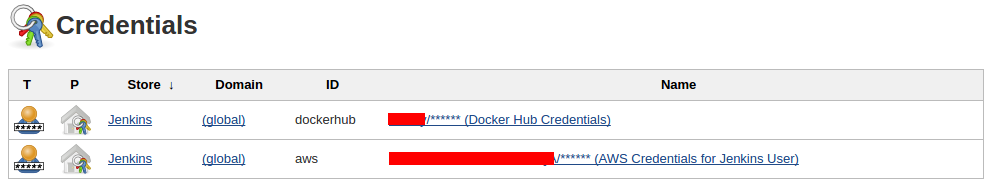
\includegraphics[width=\textwidth,keepaspectratio]{creds}
			\label{fig:creds}
		\end{figure}

	\subsection{Jenkins Job}
	The last step was to create the Jenkins job. This was created and configured on the Jenkins console. Configuration of the main build steps is outlined below.
	

		\subsubsection{Cloning the Source Code}
		The URL for the repo containing the source code was configured. Credentials can be configured for pulling from a private repo. However, the source code for the app is contained in a public repo so credentials are not needed.
		
		\begin{figure}[H]
			\caption{Source Code Management}
			\centering
			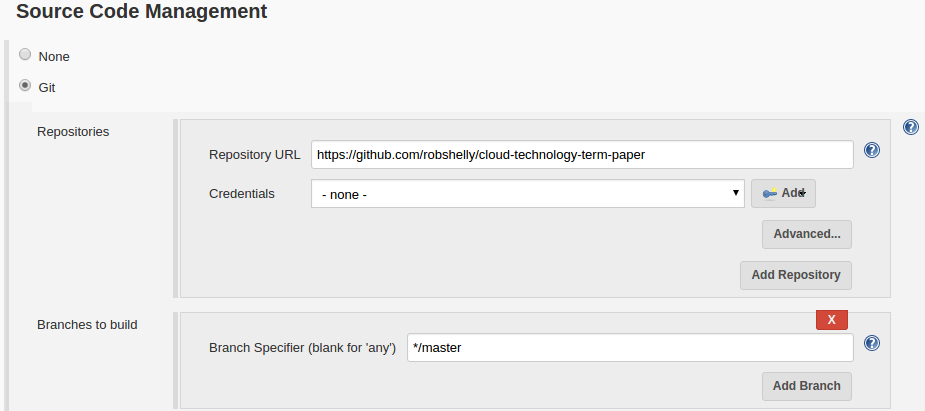
\includegraphics[width=\textwidth,keepaspectratio]{scm}
			\label{fig:scm}
		\end{figure}
	
		\subsubsection{Build and Push Image}
		This step was possible using the Docker Build and Publish Plugin. To configure it, the repository name for the image was entered. The Tag for the image is configured as a version number created using the BUILD\_NUMBER argument. This argument is made available to the Jenkins job and corresponds to the build number of the jenkins job. The credentials for the Docker Registry are also provided, allowing the image to be pushed to the registry.
		
		\begin{figure}[H]
			\caption{Docker Build}
			\centering
			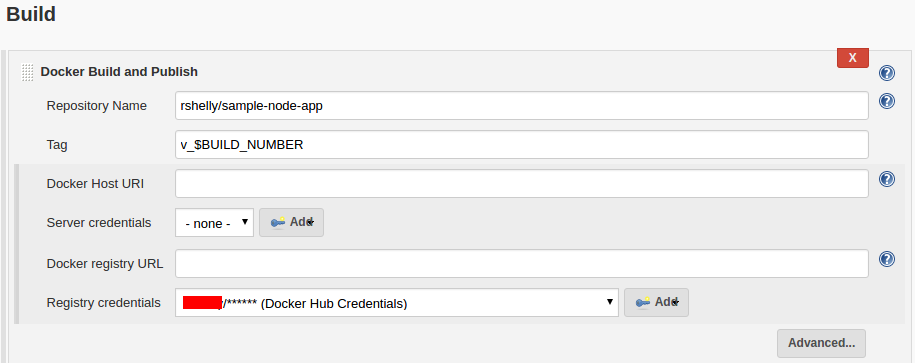
\includegraphics[width=\textwidth,keepaspectratio]{image-build}
			\label{fig:image-build}
		\end{figure}
	
		\subsubsection{Shell Script}
		The final step of the build is a shell script. This takes care of deploying the image to AWS.
		
		\begin{minipage}{\textwidth}
		\begin{lstlisting}[caption={Shell Script},label=shell-script,language=bash]
		SERVICE_NAME="node-app-service"
		IMAGE_VERSION="v_"${BUILD_NUMBER}
		TASK_FAMILY="node-app"
		CLUSTER_NAME="node-app-cluster"
		
		# Create a new task definition for this build
		sed -e "s;%BUILD_NUMBER%;${BUILD_NUMBER};g" /home/ubuntu/app/node-app.json > node-app-v_${BUILD_NUMBER}.json
		AWS_ACCESS_KEY_ID=$KEY_ID AWS_SECRET_ACCESS_KEY=$SECRET_KEY aws ecs --region eu-west-1 register-task-definition --family $TASK_FAMILY --cli-input-json file://node-app-v_${BUILD_NUMBER}.json
		
		# Update the service with the new task definition and desired count
		TASK_REVISION=`AWS_ACCESS_KEY_ID=$KEY_ID AWS_SECRET_ACCESS_KEY=$SECRET_KEY aws ecs --region eu-west-1 describe-task-definition --task-definition $TASK_FAMILY | egrep "revision" | tr "/" " " | awk '{print $2}' | sed 's/"$//'`
		DESIRED_COUNT=`AWS_ACCESS_KEY_ID=$KEY_ID AWS_SECRET_ACCESS_KEY=$SECRET_KEY aws ecs --region eu-west-1 describe-services --services ${SERVICE_NAME} --cluster $CLUSTER_NAME | egrep -m 1 "desiredCount" | tr "/" " " | awk '{print $2}' | sed 's/,$//'`
		if [ ${DESIRED_COUNT} = "0" ]; then
		DESIRED_COUNT="1"
		fi
		
		AWS_ACCESS_KEY_ID=$KEY_ID AWS_SECRET_ACCESS_KEY=$SECRET_KEY aws ecs --region eu-west-1 update-service --cluster $CLUSTER_NAME --service ${SERVICE_NAME} --task-definition ${TASK_FAMILY}:${TASK_REVISION} --desired-count ${DESIRED_COUNT}
		\end{lstlisting}
		\end{minipage}
		
		The actions performed by the shell script can be summarised as follow:
		\begin{enumerate}
			\item From the task definition template, create a new task definition specifying the latest image version;
			\item Register the new task definition;
			\item Query the task definition for the Revision Number of the latest registered definition.
			\item Query the service to find the number of desired tasks (this step would accommodate cases where autoscaling/load balancing are implemented, finding out the current number of tasks and ensuring the same number of updated tasks are started);
			\item Update the service to start the correct number of the tasks defined by the latest revision.
		\end{enumerate}
		Notice the use of the KEY\_ID and SECRET\_KEY variables in the \hyperref[shell-script]{shell script}. These are the AWS credentials that were added to Jenkins. They are made available to the job via these variable names in the job configuration.
		
		\begin{figure}[H]
			\caption{AWS Credentials}
			\centering
			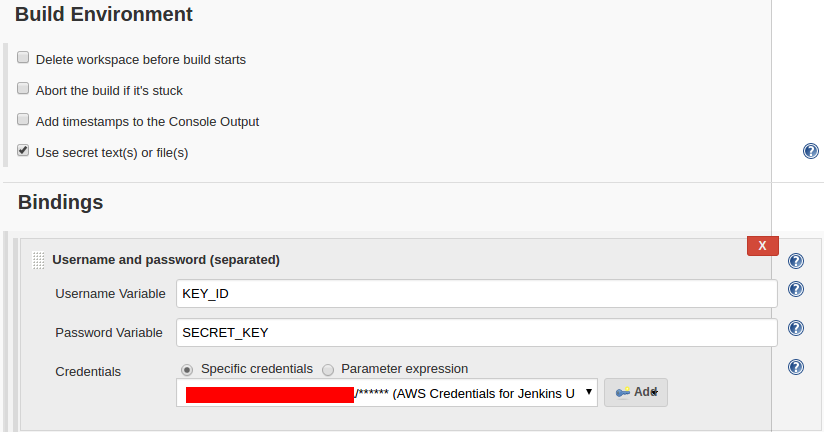
\includegraphics[width=\textwidth,keepaspectratio]{aws-creds}
			\label{fig:aws-creds}
		\end{figure}

	\section{Running the Job}
	Once all the infrastructure was created and the Jenkins job configured the CI/CD of the web app could be demonstrated. To do this a change was made to the app's source code. The changes where then committed and push to GitHub using Git. A job was immediately observed starting on the Jenkins server. Once the job was finished the app could be viewed by visiting the DNS of the EC2 instance. \autoref{fig:success} shows the successful results of a number a jobs, i.e. the various versions of the image on Docker Hub and the app running on the 
	
	\begin{figure}[H]
		\caption{CI/CD in Action}
		\centering
		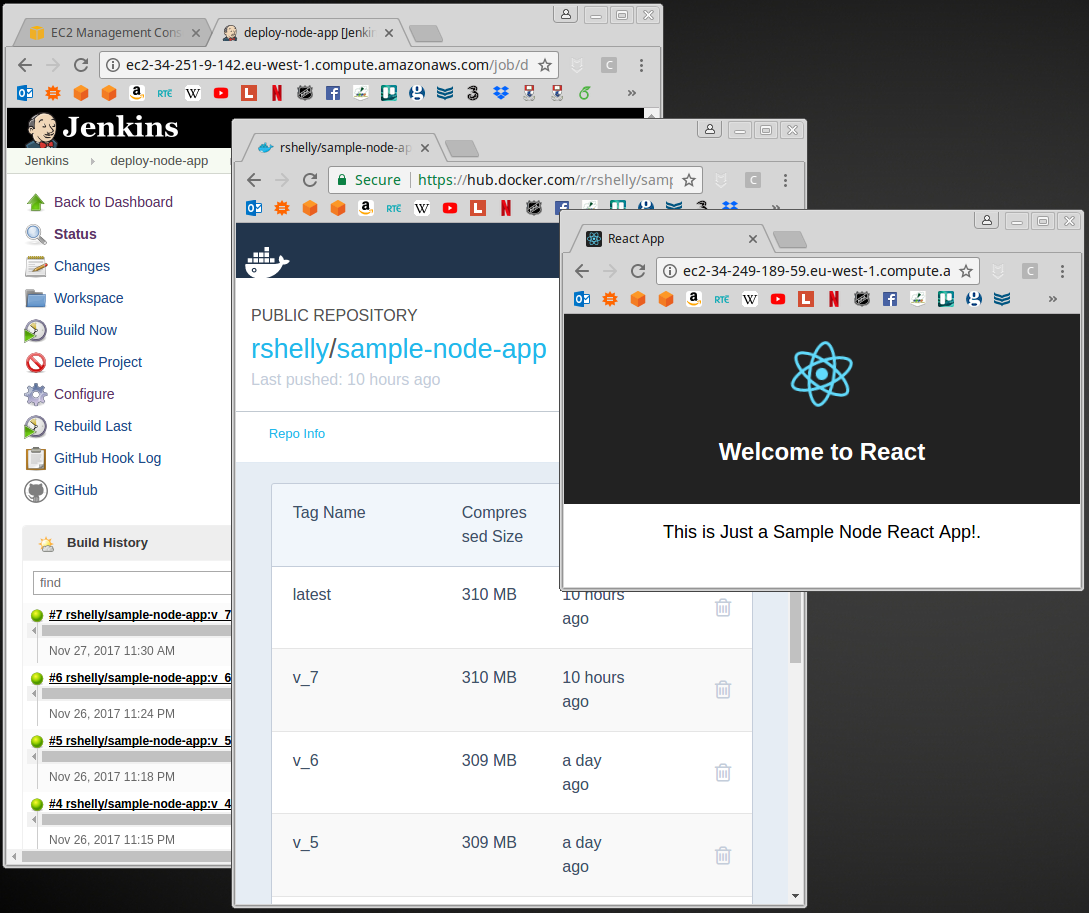
\includegraphics[width=\textwidth,keepaspectratio]{success}
		\label{fig:success}
	\end{figure}
	
	